\documentclass[a4paper, 12pt]{article}

\usepackage[english,russian]{babel}
\usepackage[T2A]{fontenc}
\usepackage[utf8]{inputenc}
\usepackage{geometry}
\usepackage{enumitem}
\usepackage{setspace}
\usepackage{amssymb}
\usepackage{graphicx}
\usepackage{wrapfig}
\usepackage{float}
\usepackage{amsmath}
\usepackage{textcomp}
\usepackage{dsfont}

\geometry{top=5mm, left=1cm}
%\setlength{\parindent}{0}
\renewcommand{\arraystretch}{1.2}
\linespread{1}

\begin{document}
    \begin{center}
        \textbf{Сферическая геометрия}\\
        Конспект
    \end{center}

    \begin{enumerate}
        \item[I.] Существует единственная прямая, проходящая через две данные различные точки,
        кроме случая, когда эти точки противоположны; тогда таких прямых бесконечно много.
        \item[II.] Существует единственный перпендикуляр к данной прямой, проходящий через данную точку,
        кроме случая, когда точка является полюсом этой прямой;
        тогда таких перпендикуляров бесконечно много.
        \item[III.] Существует единственная окружность с данным центром $O'$ и данным радиусом $\rho$,
        если, $0 < \rho < \dfrac{\pi}{2}$ где $R$ - радиус сферы.
        \item[IV.] Для каждой точки на прямой и каждого положительного числа существуют ровно две точки на этой прямой,
        расстояния от которых до данной точки равны данному числу,
        если только это число меньше $\pi R$, где R - радиус сферы.
        \item[V.] Любые две прямые пересекаются в двух диаметрально противоположных точках.
    \end{enumerate}

    \begin{minipage}[t]{0.25\textwidth}
        \begin{center}
            \textbf{Сфера}
            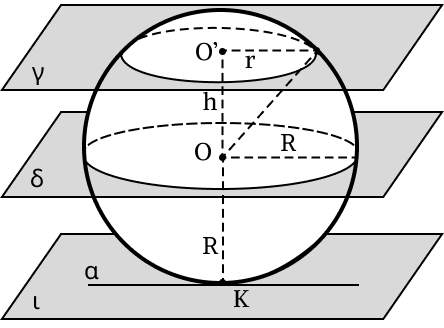
\includegraphics[width=1\linewidth]{images/img1}\\
        \end{center}
        \begin{flushleft}
            Сфера $(O;R)$
            $S = 4\pi R ^2$ \\ \

            Окружность$(O';r)$ - малая окружность\\ \

            Окружность$(O;R)$ - большая окружность\\ \

            $C=2\pi R$\\
            $C_\alpha = \alpha R$\\ \

            $\iota, \alpha$ - касательные

        \end{flushleft}
    \end{minipage}
    \begin{minipage}[t]{0.25 \textwidth}
        \begin{center}
            \textbf{Прямые}
            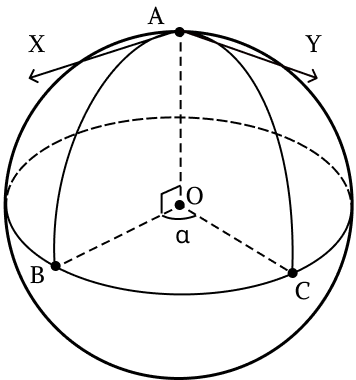
\includegraphics[width=0.7\linewidth]{images/img2}\\
        \end{center}
        \begin{flushleft}
            Угол:\\
            $BO$\textasciicircum$CO=\angle BOC = X$\textasciicircum$Y = (BOA)$\textasciicircum$(COA)$
        \end{flushleft}\\ \

        Расстояние:\\
        $\rho(B;C) = \alpha R$


    \end{minipage}
    \begin{minipage}[t]{0.25 \textwidth}
        \begin{center}
            \textbf{Двуугольник}
            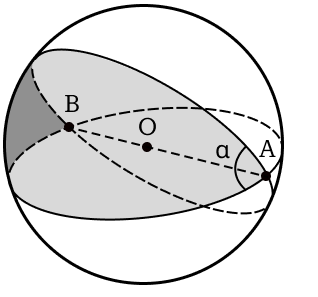
\includegraphics[width=0.8\linewidth]{images/img3}\\
        \end{center}
        Площадь:\\
        $2\alpha r^2$
    \end{minipage}
    \begin{minipage}[t]{0.25\textwidth}
        \begin{center}
            \textbf{Треугольник}
            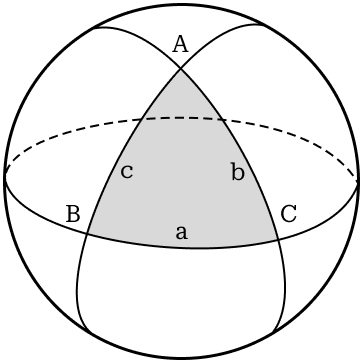
\includegraphics[width=0.75\linewidth]{images/img4}\\
        \end{center}
        Теорема синусов:\\
        $\dfrac{\sin\frac{a}{R}}{\sin A} = \dfrac{\sin\frac{b}{R}}{\sin B} = \dfrac{\sin\frac{c}{R}}{\sin C}$\\

        Теорема косинусов:
        \begin{spacing}{1.2}
            $\cos\frac{a}{R} = \cos\frac{b}{R}\cos\frac{c}{R} + \sin\frac{b}{R}\sin\frac{c}{R}\cos A$
        \end{spacing}\

        Теорема Пифагора:\\
        $\cos\frac{a}{R}=\cos\frac{b}{R}\cos\frac{c}{R}$\\

        Площадь:\\
        $S(\triangle ABC)=\\r^2(A + B + C - \pi)$

    \end{minipage}\\ \ \\

    \textbf{Изометрия} - биекция $\beta$, для которой при функции расстояния $d(A, B)$ для каждой точки
    пространства верно $d(\beta(A), \beta(B)) = d(A, B)$\\

    \textbf{Движение} - собственная изометрия, то есть изометрия при которой сохраняется ориентация.

\end{document}
